% --- Recommended figure (model choice / eval workflow narrative) ---
% Best match in visualizations/out/: experiment_protocol_baseline_vs_sft.png
% (baseline vs SFT protocol). For splits-only emphasis, use train_dev_test_schematic.png
% Few-shot rollup heatmaps + metric definitions + backbone choice: baseline_few_shot_selection.png
% 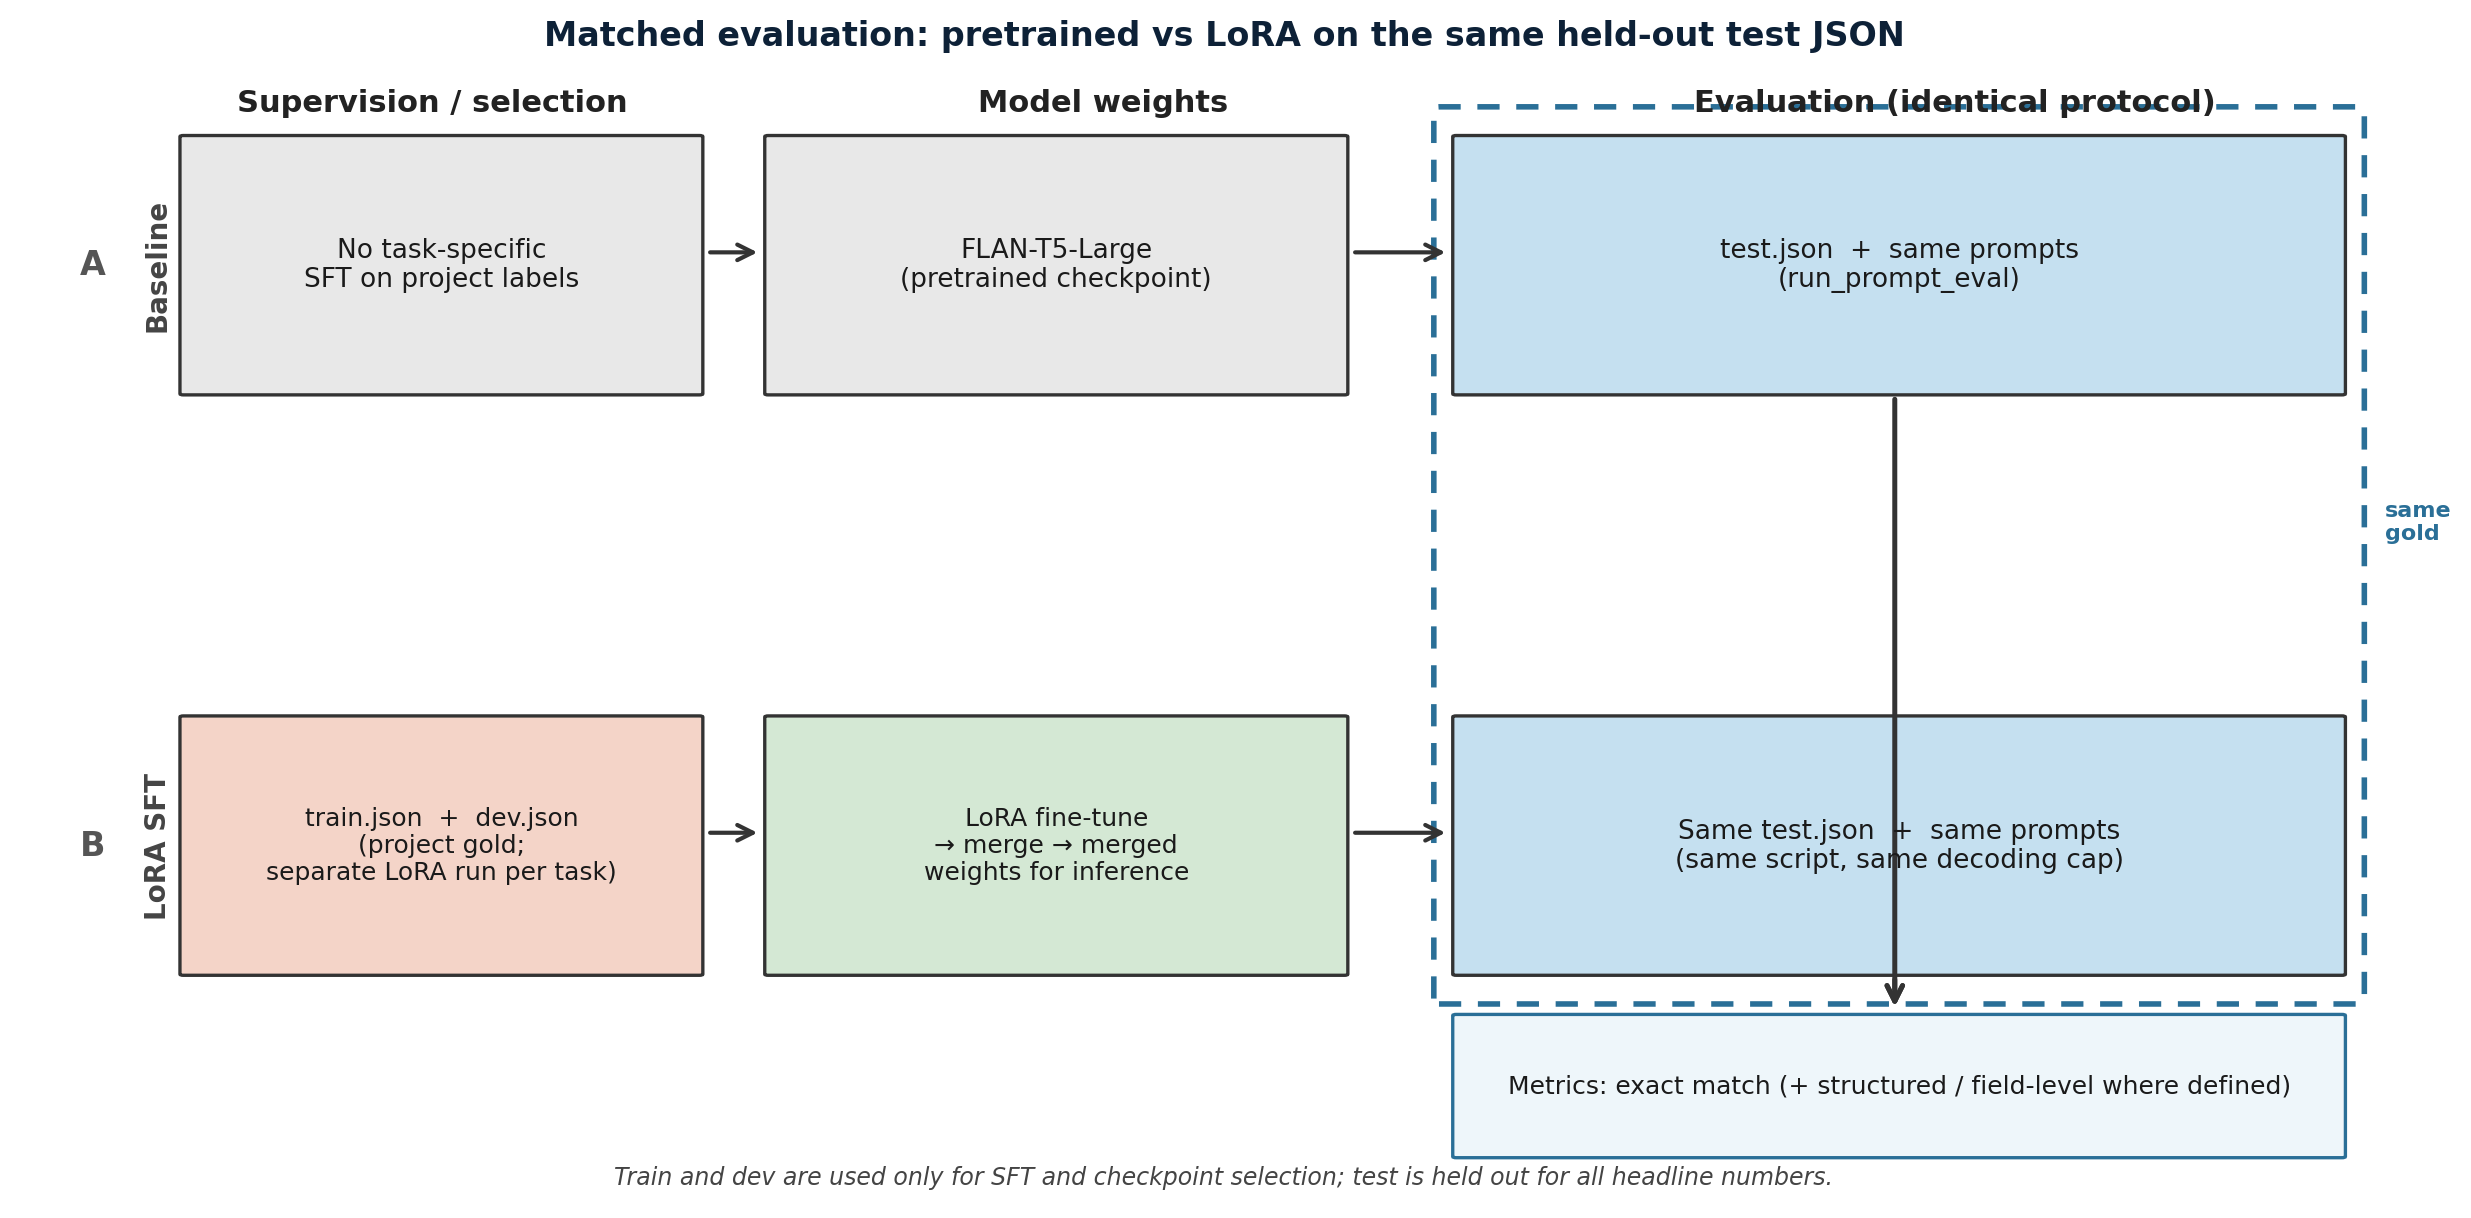
\includegraphics[width=\linewidth]{../visualizations/out/experiment_protocol_baseline_vs_sft}

% Rationale for three supervised tasks (no natural_text in thesis runs): see OVERVIEW.MD
% "Research goals and experimental design" — formal stuckness (Generative Aesthetics),
% isolability of meter vs rhyme, joint combined condition + Caruana/Ruder/Liu vs Standley et al.

% =============================================================================
% Opening paragraph (evaluation phase + compute; three task conditions)
% =============================================================================

After the corpus has been constructed and annotated, the evaluation phase establishes reproducible splits, prepares task-specific datasets for three supervised objectives, and scores prompt-only baselines to guide model selection.
We do \emph{not} use the separate \texttt{natural\_text} continuation task in this thesis track: the research question is whether \emph{explicit} formal supervision (meter, rhyme, and their joint bundle) changes behavior relative to the same backbone and eval harness, not whether the model can continue raw verse in an open-ended way.
The evaluation code under \texttt{evaluation/} is a small set of CLIs (splits, annotation coverage, rollup) plus \texttt{scripts/run\_prompt\_eval.py} for inference.
Most steps operate only on SQLite and JSON and can run locally or on a login node; neural baselines are submitted as batch jobs (CPU or GPU depending on script and model size).
After inference, gold annotation coverage and model scores are aggregated for comparison (\texttt{evaluation/annotation\_coverage.json}, \texttt{evaluation/baseline\_report/model\_comparison.csv}).

% =============================================================================
\section{Experimental Setup}
% =============================================================================

\paragraph{Why meter, rhyme, and combined (and not natural text here).}
Prior work on LLM verse (\emph{Generative Aesthetics: On formal stuckness in AI verse}) documents \emph{formal stuckness}: models drift toward frequent meters and end-rhyme even when asked not to---suggesting surface statistics rather than flexible control.
This project therefore stresses \textbf{verifiable} targets: \texttt{meter\_only} and \texttt{rhyme\_only} give \textbf{isolable} objectives (attribution and negative-transfer checks; cf.\ Standley et al.\ on which tasks to train jointly), while \texttt{combined} matches how annotations co-occur in the corpus and probes \textbf{compositionality} of multi-field decoding (cf.\ multitask-learning motivation in Caruana; Ruder; Liu et al.; see OVERVIEW.MD for full citations).
\texttt{natural\_text} remains in the repository for ablations, but the headline experiments are the three formal conditions above.

\paragraph{Step 1: Evaluation Splits.}
Author metadata supports two explicit holdouts: \texttt{held\_out\_poets} reserves \emph{all} poems by up to ten randomly chosen authors with at least three poems each (unseen authors), and \texttt{held\_out\_poems} samples a fixed number of poems (default 100) from the remaining pool.
\textbf{Train/dev/test} are not stratified per author; after those holdouts, remaining poem IDs are \textbf{shuffled once} (fixed seed \texttt{RANDOM\_SEED = 42} in \texttt{evaluation/corpus/splits.py}) and partitioned \textbf{70/15/15} into train, dev, and test.
Author-level leakage for the main split is controlled primarily by the poet holdout set, not by the 70/15/15 partition itself.

\paragraph{Step 2: Dataset Preparation (three conditions).}
Task-specific JSON is prepared for \texttt{meter\_only}, \texttt{rhyme\_only}, and \texttt{combined}.
For \textit{meter\_only}, the input is the line text and the target is the gold stress pattern as \texttt{+}/\texttt{-} symbols.
For \textit{rhyme\_only}, the target is a compact rhyme key from per-word ARPAbet phonology, with fallback to the line's Poesy \texttt{rhyme\_group} when the key is empty.
For \textit{combined}, the input follows the continuation pattern (prior line or \texttt{[start]}); the target bundles stress, \texttt{meter\_type}, rhyme, end-stopping, and caesura in a fixed pipe-delimited schema, with \texttt{next\_line} for strict alignment at eval time.

\paragraph{Step 3: Prompt-Only Baselines.}
\texttt{scripts/run\_prompt\_eval.py} loads each test split, builds zero/one/few-shot prompts, and calls Hugging Face Transformers (seq2seq vs causal LM as appropriate).
Slurm templates submit per-model jobs; CPU baselines use \texttt{--device -1} in \texttt{baseline\_cpu.slurm}; larger models typically use GPU nodes.

\paragraph{Step 4: Coverage and Scoring.}
\textit{(a)} \texttt{evaluation/run\_annotation\_coverage.py} reports gold annotation completeness per split into \texttt{evaluation/annotation\_coverage.json}.
\textit{(b)} Model JSON is scored vs.\ gold (exact match, structured fields for \textit{combined}, optional Levenshtein in rollup) via \texttt{evaluation/summarize\_prompt\_baselines.py} $\rightarrow$ \texttt{evaluation/baseline\_report/model\_comparison.csv}.

% Requires \usepackage{booktabs} in the preamble.
\begin{table}[t]
  \centering
  \small
  \caption{Prompt-only baselines under \textbf{few-shot} prompting (default templates in \texttt{scripts/run\_prompt\_eval.py}). Exact match (EM) and normalized string similarity (Sim, \%) from \texttt{evaluation/baseline\_report/model\_comparison.csv}; $n=500$ scored lines per task. On \texttt{meter\_only}, FLAN-T5-Large in \textbf{zero-shot} on the same cap remains at EM $0\%$ / Sim $\approx 14.7\%$, so the discriminative signal here is primarily few-shot ICL.}
  \label{tab:baseline-fewshot-summary}
  \begin{tabular}{@{}llrrrrrr@{}}
    \toprule
    & & \multicolumn{2}{c}{\texttt{meter\_only}} & \multicolumn{2}{c}{\texttt{rhyme\_only}} & \multicolumn{2}{c@{}}{\texttt{combined}} \\
    \cmidrule(lr){3-4} \cmidrule(lr){5-6} \cmidrule(lr){7-8}
    Model & Arch. & EM & Sim & EM & Sim & EM & Sim \\
    \midrule
    FLAN-T5-Large & enc--dec & 44.0 & 82.9 & 0.4 & 43.7 & 0.0 & 63.1 \\
    BART-large & enc--dec & 0.0 & 4.9 & 0.0 & 2.3 & 0.0 & 46.2 \\
    GPT-2-medium & causal & 0.0 & 1.7 & 0.0 & 2.3 & 0.0 & 62.5 \\
    GPT-2 & causal & 0.0 & 1.1 & 0.0 & 3.0 & 0.0 & 44.2 \\
    Phi-2 & causal & 0.0 & 2.4 & 0.0 & 2.0 & 0.0 & 43.9 \\
    \bottomrule
  \end{tabular}
\end{table}

\paragraph{Step 5: Model Selection.}
Metrics, runtime, and memory jointly determine which backbone proceeds to LoRA fine-tuning on the same three tasks.

\paragraph{Execution Environment.}
Corpus, splits, and \texttt{output/training\_data/} are built locally; baselines run on the cluster; rollups return to a local or login node for selection.
